\textbf{Danke an ...}

%TODO: Tutorennamen hier einfügen
Tutor1, Tutor2, Tutor3, ...

\addchap{Vorwort}

%TODO: neues Vorwort hier einfügen

Hallo Uniwelt!

heißt es nun für dich als frisch Immatrikulierter, Ersti, an der TU Dresden. 
Endlich kannst du nach Jahren der Knechtschaft selbst über dich und dein Leben bestimmen. 
Wie du mit dieser Freiheit und der daraus folgenden Verantwortung zurecht kommst, lernst du schnell. 
Damit dir der Übergang leichter fällt, veranstaltet dein Fachschaftsrat die Erstsemestereinführung (ESE). 
Eine Woche lang gibt es neben Spiel und Spaß sehr viel Informatives zum Studium sowie zum Unileben allgemein. 
Dieses Heft ist ein nützlicher Ratgeber und nicht vergessen: 
NO PANIC! (aus historischen Gründen hier nicht das grammatikalisch korrekte \glqq don't panic\grqq)

Du wirst auch entdecken, dass Uni mehr ist als nur studieren. 
Neben allerlei Erstemesterparties gibt es noch mehr zu erleben. 
Prägend für die Dresdner Hochschulkultur sind das studentische Kino im Klub Neue Mensa sowie die 15 Studentenclubs, wie z.B. das CountDown. 
In der Neustadt laden viele Kneipen und Clubs zu langen Nächten ein. 
Einmal im Jahr entlädt sich dieses alternative Flair während der BRN (Bunte Republik Neustadt). 
Und wem das alles viel zu hektisch ist: der fläze sich gemütlich in ein Sofa vom ASCII, dem Studentencafé der Fakultät. 
Dort kann man gut bei Kaffee und Club Mate (empfehlenswert auch die lokale Kolle-Mate!) entspannen oder versuchen doch etwas für die Uni zu tun.

Engagement wird an der TU Dresden groß geschrieben. 
Es gibt viele Hochschulgruppen die um eure Mitarbeit buhlen. 
Darunter einige politische, wie auch technische, journalistische, künstlerische und und und. Mehr dazu findest du auf der Seite des StuRa.

\textbf{Zu guter Letzt: Wir (ESE-Tutoren) wünschen Dir viel Erfolg beim Studium!}

\begin{figure}
\centering 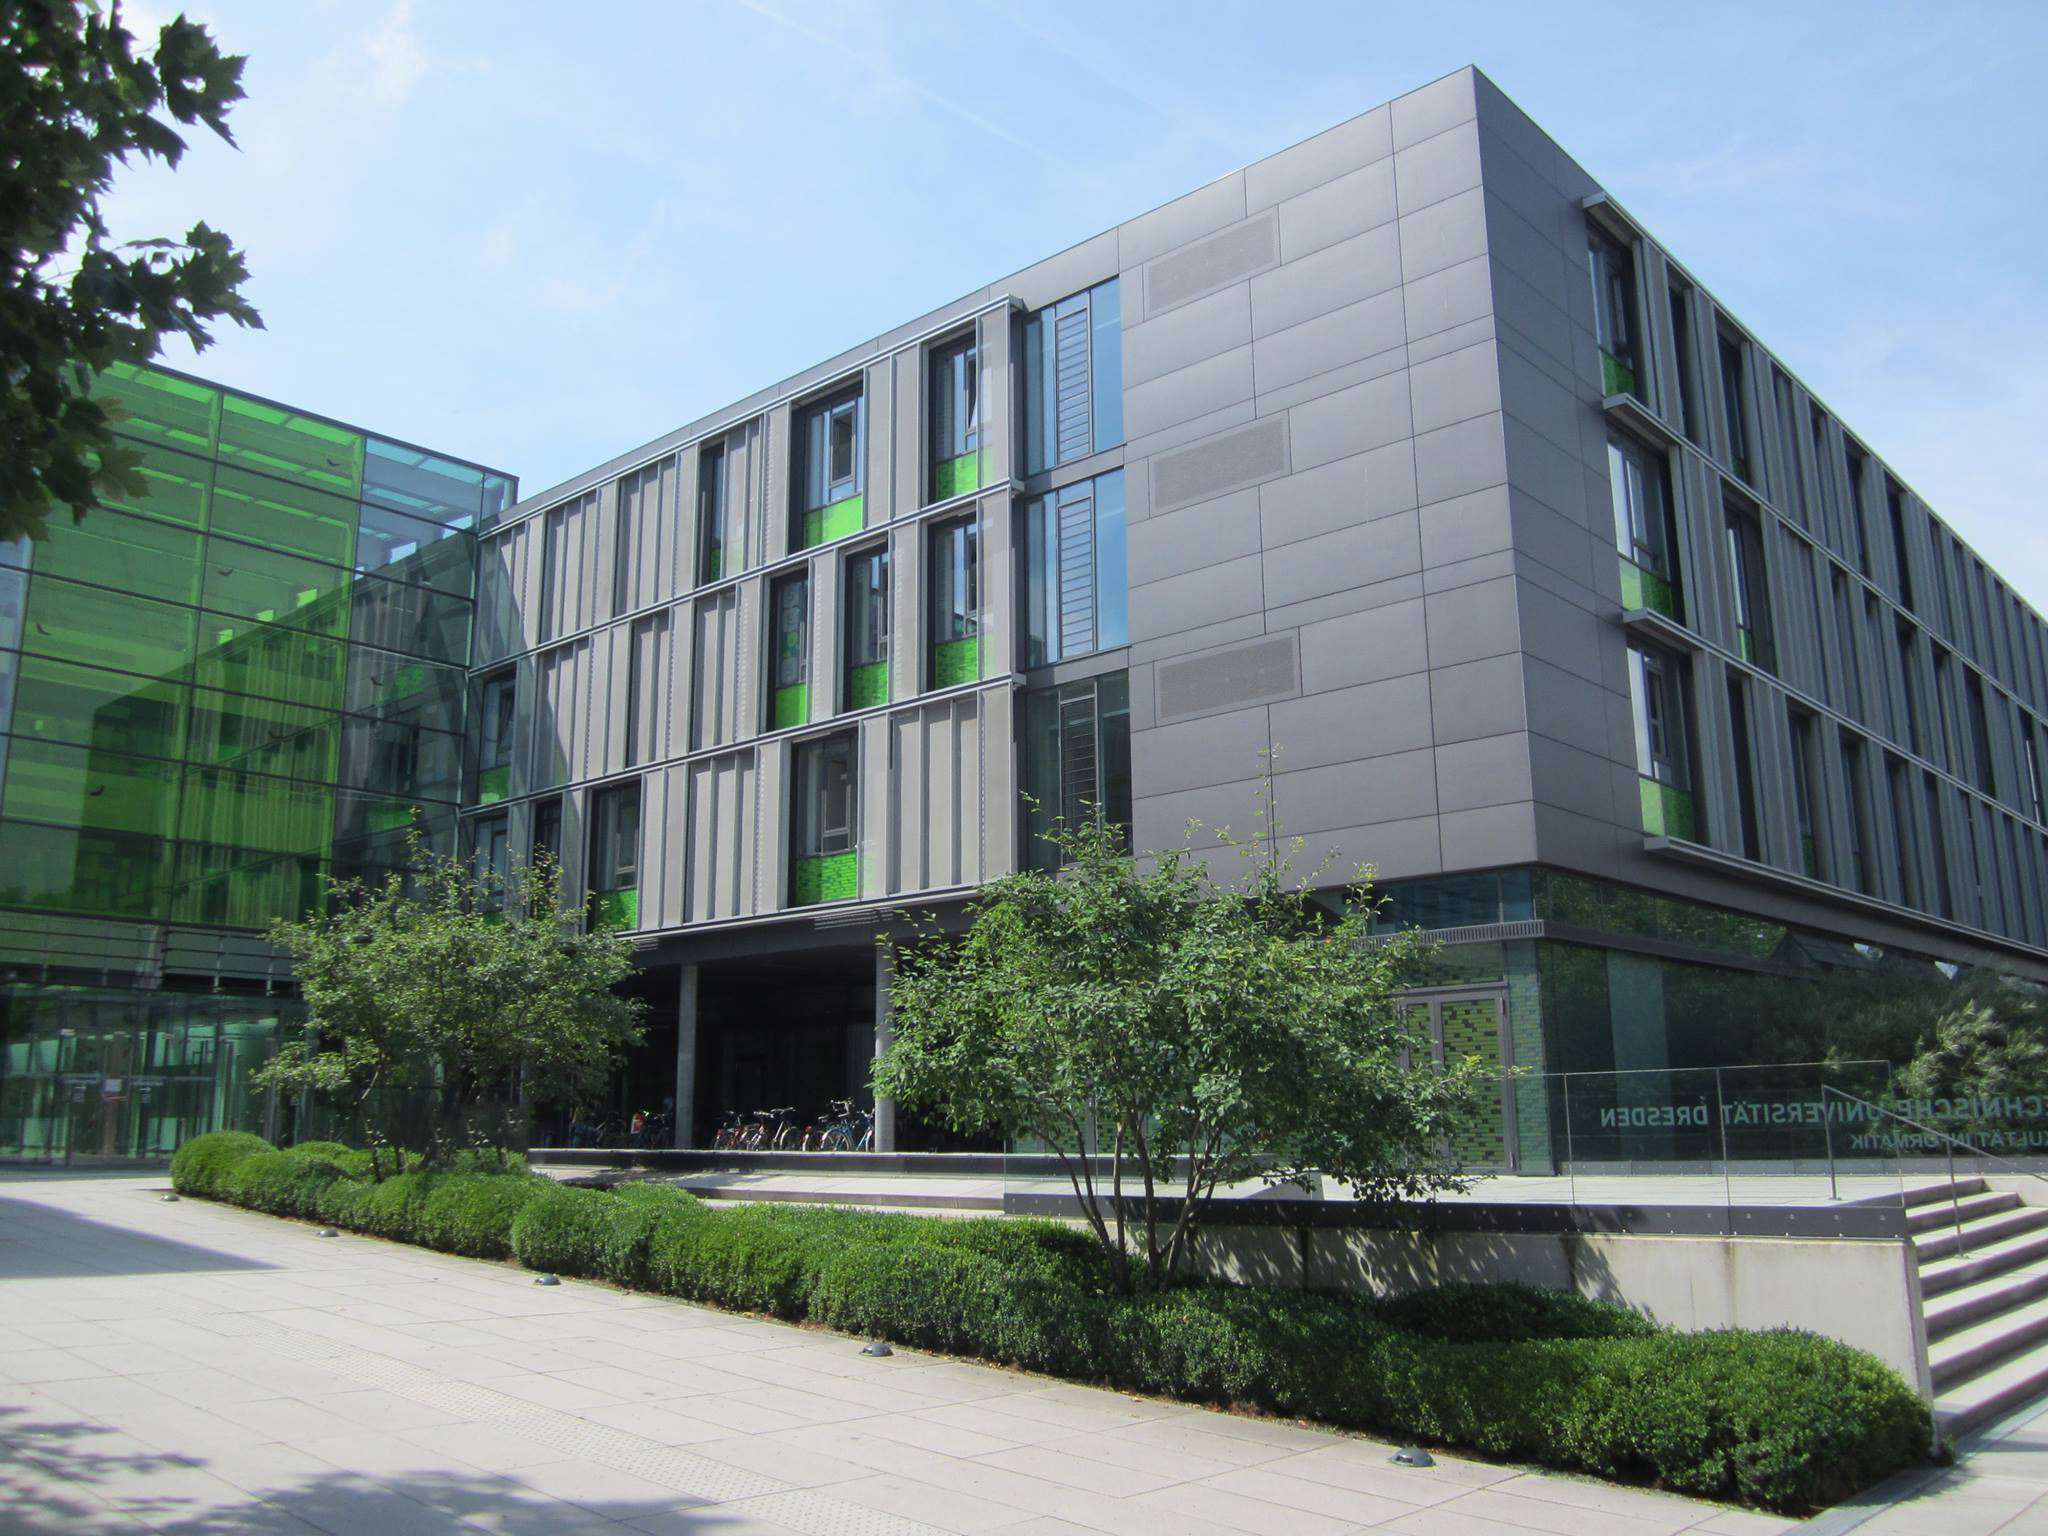
\includegraphics[width=\linewidth]{img/fakultaet.jpg}
\caption*{{\small Fakultät Informatik - Foto: Hb3 (CC-BY-SA)}}
\end{figure}
%Bildlink: http://commons.wikimedia.org/wiki/File:TU-Dresden-Informatik.jpg
